\section{ハーフ・ポジション}
\begin{center}
\begin{tabular}{|lcl|}
\hline
この章の基礎練習 & : & 開放弦の練習\\ 
この章の修了課題 & : & 1. 「\ref{half_scale}」の音階練習を正しい音程で暗譜して演奏できる\\
               &   & 2. サン=サーンスの「亀」を正しい音程で暗譜して演奏できる\\
\hline
\end{tabular}
\end{center}

\subsection{ハーフ・ポジションの位置}
 ハーフ・ポジションはネックの上端にあるポジションです(図\addtocounter{figure}{2}\thefigure 、 
\addtocounter{figure}{1}\thefigure)。ハーフ・ポジションの4の指は第IIポジションの1の場所を押さえます。%親指は2の指の裏側に置きます(図\addtocounter{figure}{1}\thefigure)。

\begin{flushleft}
\begin{minipage}{80pt}
\addtocounter{figure}{-2}
\begin{center}
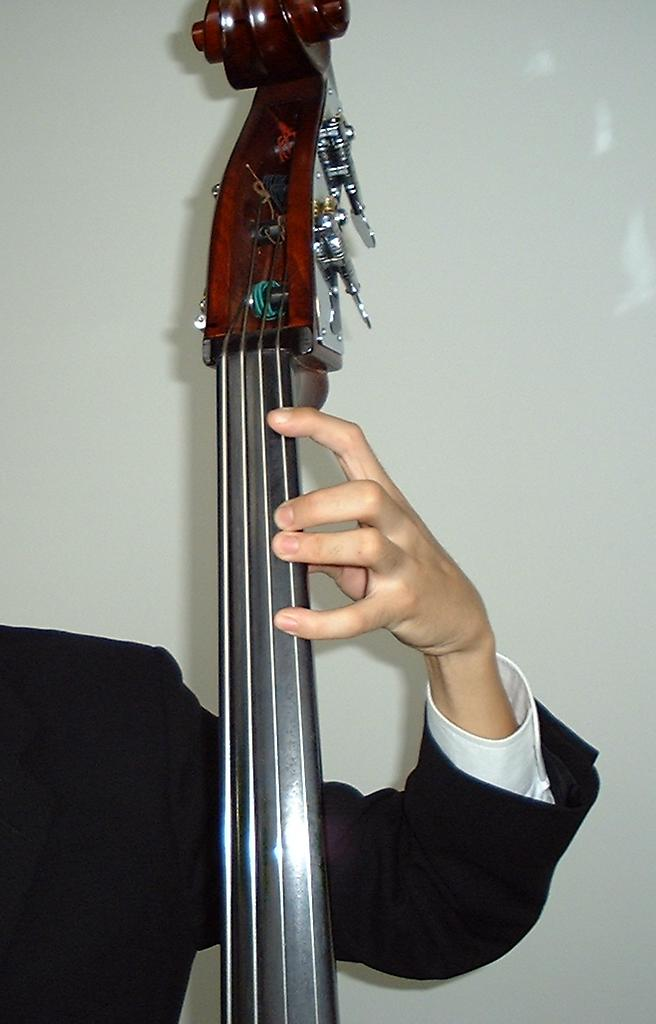
\includegraphics[height=4.3cm]{Pics/Position/half_1.epsi}\\
\end{center}
{\small 図\thefigure : ハーフ・ポジションの位置\\}
\end{minipage}
\hfill
\begin{minipage}{80pt}
\addtocounter{figure}{1}
\begin{center}
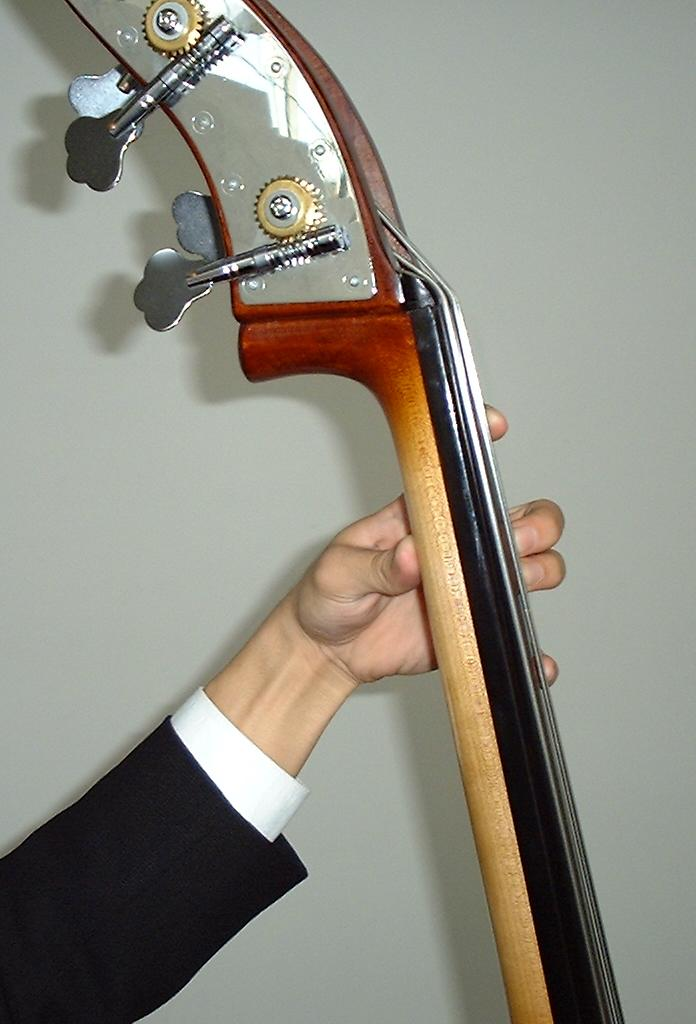
\includegraphics[height=4.3cm]{Pics/Position/half_3.epsi}\\
\end{center}
{\small 図\thefigure : 奏者から見たハーフ・ポジション}\\
\end{minipage}
\hfill
\begin{minipage}{85pt}
\addtocounter{figure}{1}
\begin{center}
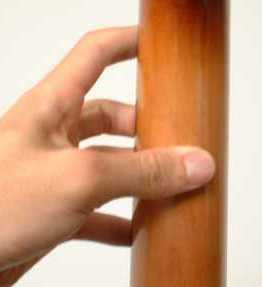
\includegraphics[height=4.3cm]{Pics/photo0830/left_thumb1.epsi}\\
\end{center}
{\small 図\thefigure : 左手親指の位置   }\\
\end{minipage}
\end{flushleft}
\indent 1の指はネックの上側に少し傾け、指のやや側面寄りの位置で押さえます(図
\addtocounter{figure}{3}\thefigure)。 

\subsection{ハーフ・ポジションで取れる音}
ハーフ・ポジションではそれぞれの弦で以下の音を取ることができます。正し
い場所を押さえているかどうか、チューニングメーターで確認しながら弾いてみましょう。\\

\begin{music}
\nostartrule
\parindent 0pt
\setclef1{\bass}  
\startpiece
\notes\enotes
\Notes\zchar{16}{G線}\zchar{11}{\bf 1}\wh{'^G}\zchar{11}{\bf 2}\wh{!=a}\zchar{11}{\bf 4}\wh{^a}\enotes
\doublebar
\Notes\zchar{11}{\bf 1}\wh{_a}\zchar{11}{\bf 2}\wh{=a}\zchar{11}{\bf 4}\wh{_b}\enotes
\doublebar
\Notes\zchar{16}{D線}\zchar{9}{\bf 1}\wh{'^D}\zchar{9}{\bf 2}\wh{E}\zchar{9}{\bf 4}\wh{F}\enotes
\doublebar
\Notes\zchar{9}{\bf 1}\wh{'_E}\zchar{9}{\bf 2}\wh{=E}\zchar{9}{\bf 4}\wh{F}\enotes
\setdoublebar
\endpiece
\startpiece
\notes\enotes
\Notes\zchar{14}{A線}\zchar{9}{\bf 1}\wh{'^A}\zchar{9}{\bf 2}\wh{B}\zchar{9}{\bf 4}\wh{C}\enotes
\doublebar
\Notes\zchar{9}{\bf 1}\wh{'_B}\zchar{9}{\bf 2}\wh{=B}\zchar{9}{\bf 4}\wh{C}\enotes\doublebar
\Notes\zchar{14}{E線}\zchar{9}{\bf 1}\wh{F}\zchar{9}{\bf 2}\wh{^F}\zchar{9}{\bf 4}\wh{G}\enotes
\doublebar
\Notes\zchar{9}{\bf 1}\wh{F}\zchar{9}{\bf 2}\wh{_G}\zchar{9}{\bf 4}\wh{G}\enotes
\setdoublebar
\endpiece
\end{music}

\subsection{音階練習 \label{half_scale}}
\begin{music}
\nostartrule
\parindent 0pt
\setclef1{\bass}  
\generalmeter{\meterC}
\generalsignature{-1}    
\startpiece
\notes\zchar{14}{ヘ長調(F-dur)音階}\enotes
\NOtes\zchar{9}{\bf 1}\qu{F}\zchar{9}{\bf 4}\qu{G}\zchar{9}{\bf 0}\qu{'A}\zchar{9}{\bf 1}\qu{B}\enotes
\bar
\NOtes\zchar{9}{\bf 4}\qu{'C}\zchar{9}{\bf 0}\ql{D}\zchar{9}{\bf 2}\ql{E}\zchar{9}{\bf 4}\ql{F}\enotes
\bar
\NOtes\zchar{9}{\bf 4}\ql{'F}\zchar{9}{\bf 2}\ql{E}\zchar{9}{\bf 0}\ql{D}\zchar{9}{\bf 4}\qu{C}\enotes
\bar
\NOtes\zchar{9}{\bf 1}\qu{'B}\zchar{9}{\bf 0}\qu{A}\zchar{9}{\bf 4}\qu{!G}\zchar{9}{\bf 1}\qu{F}\enotes
\setdoublebar
\endpiece

\generalmeter{\meterC}
\generalsignature{-2}    
\startpiece
\notes\zchar{14}{変ロ長調(B-dur)音階}\enotes
\NOtes\zchar{9}{\bf 1}\qu{'B}\zchar{9}{\bf 4}\qu{C}\zchar{9}{\bf 0}\ql{D}\zchar{9}{\bf 1}\ql{E}\enotes
\bar
\NOtes\zchar{9}{\bf 4}\ql{'F}\zchar{9}{\bf 0}\ql{G}\zchar{10}{\bf 2}\ql{!a}\zchar{11}{\bf 4}\ql{b}\enotes
\bar
\NOtes\zchar{11}{\bf 4}\ql{b}\zchar{10}{\bf 2}\ql{a}\zchar{9}{\bf 0}\ql{'G}\zchar{9}{\bf 4}\ql{F}\enotes
\bar
\NOtes\zchar{9}{\bf 1}\ql{'E}\zchar{9}{\bf 0}\ql{D}\zchar{9}{\bf 4}\qu{C}\zchar{9}{\bf 1}\qu{B}\enotes
\setdoublebar\endpiece
\generalmeter{\meterC}
\generalsignature{5}    
\startpiece
\notes\zchar{18}{ロ長調(H-dur)音階}\enotes
\NOtes\zchar{14}{I}\ovbkt{!f}{1.1}{0}\zchar{9}{\bf 1}\qu{'B}\zchar{9}{\bf 4}\qu{C}\zchar{14}{half}\ovbkt{!f}{0.1}{0}\zchar{9}{\bf 1}\ql{'D}\zchar{14}{I}\ovbkt{!f}{1.4}{0}\zchar{9}{\bf 1}\ql{'E}\enotes
\bar
\NOtes\zchar{9}{\bf 4}\ql{'F}\zchar{14}{half}\ovbkt{!f}{0.1}{0}\zchar{9}{\bf 1}\ql{'G}\zchar{15}{I}\ovbkt{!g}{3.4}{0}\zchar{10}{\bf 2}\ql{!a}\zchar{11}{\bf 4}\ql{b}\enotes
\bar
\NOtes\zchar{11}{\bf 4}\ql{b}\zchar{10}{\bf 2}\ql{a}\zchar{14}{half}\ovbkt{!f}{0.1}{0}\zchar{9}{\bf 1}\ql{'G}\zchar{14}{I}\ovbkt{!f}{1.4}{0}\zchar{9}{\bf 4}\ql{'F}\enotes
\bar
\NOtes\zchar{9}{\bf 1}\ql{'E}\zchar{14}{half}\ovbkt{!f}{0.1}{0}\zchar{9}{\bf 1}\ql{'D}\zchar{14}{I}\ovbkt{!f}{1.1}{0}\zchar{9}{\bf 4}\qu{'C}\zchar{9}{\bf 1}\qu{B}\enotes
\setdoublebar\endpiece
\setclef1{\bass}  
\generalmeter{\meterC}
\generalsignature{6}    
\startpiece
\notes\zchar{18}{嬰ヘ長調(Fis-dur)音階}\enotes
\NOtes\zchar{14}{I}\ovbkt{!f}{1.1}{0}\zchar{9}{\bf 1}\qu{F}\zchar{9}{\bf 4}\qu{G}\zchar{14}{half}\ovbkt{!f}{0.1}{0}\zchar{9}{\bf 1}\qu{'A}\zchar{14}{I}\ovbkt{!f}{1.4}{0}\zchar{9}{\bf 1}\qu{'B}\enotes
\bar
\NOtes\zchar{9}{\bf 4}\qu{'C}\zchar{14}{half}\ovbkt{!f}{0.1}{0}\zchar{9}{\bf 1}\ql{'D}\zchar{15}{I}\ovbkt{!g}{3.4}{0}\zchar{9}{\bf 1}\ql{'E}\zchar{9}{\bf 4}\ql{F}\enotes
\bar
\NOtes\zchar{9}{\bf 4}\ql{'F}\zchar{9}{\bf 1}\ql{E}\zchar{14}{half}\ovbkt{!f}{0.1}{0}\zchar{9}{\bf 1}\ql{'D}\zchar{14}{I}\ovbkt{!f}{1.4}{0}\zchar{9}{\bf 4}\qu{'C}\enotes
\bar
\NOtes\zchar{9}{\bf 1}\qu{'B}\zchar{14}{half}\ovbkt{!f}{0.1}{0}\zchar{9}{\bf 1}\qu{'A}\zchar{14}{I}\ovbkt{!f}{1.1}{0}\zchar{9}{\bf 4}\qu{!G}\zchar{9}{\bf 1}\qu{F}\enotes
\setdoublebar\endpiece
\end{music}

\subsection{ハーフ・ポジションで弾ける名曲}
\subsubsection*{ワーグナー: 楽劇「ニュルンベルクのマイスタージンガー」 第1幕への前奏曲より}
\begin{music}
\nostartrule
\setclef1{\bass}
\generalsignature{0}    
\generalmeter{\meterfrac44}
\parindent 0pt
\startbarno=158
\def\writebarno{\tenrm\the\barno\barnoadd}
\def\raisebarno{2\internote}
\def\shiftbarno{0.1\Interligne}
\systemnumbers
\startpiece\bigaccid
\notes\zchar{18}{\LARGE \bf J}\zchar{20}{\hspace{2em} \bf aber sehr markiert}\zchar{16}{\hspace{2em}({\it ma molto marcato})}\enotes
\NOtes\zchar{-4}{I}\zchar{-8}{\mf}\zchar{12}{\downbow}\zchar{10}{\bf 2}\hu{'C}\zchar{10}{\upbow}\qup{!G}\zchar{8}{\upbow}\cu{!G}\enotes
\bar
\NOtes\islurd{0}{G}\zchar{8}{\downbow}\hu{G}\enotes
\notes\ibu{0}{G}{0}\tslur{0}{G}\qb{0}{GE}\zchar{-6}{half}\zchar{8}{\bf 1}\qb{0}{F}\tbu{0}\qb0{G}\enotes
\bar 
\Notes\zchar{-4}{I}\qu{'A}\zchar{8}{\bf 1}\qu{B}\qu{C}\zchar{8}{\bf 0}\ql{D}\enotes
\bar
\Notes\zchar{10}{\downbow}\zchar{8}{\bf 1}\ql{'E}\isluru{0}{F}\zchar{8}{\downbow}\ql{F}\enotes
\notes\ibl{0}{'F}{-3}\tslur{0}{F}\qb{0}{FE}\zchar{-6}{II}\zchar{8}{\bf 4}\qb{0}{D}\tbl{0}\zchar{8}{\bf 1}\qb{0}{C}\enotes
\bar
\NOtes\zchar{11}{\downbow}\zchar{8}{\bf 4}\hl{'D}\zchar{11}{\upbow}\zchar{8}{\bf 4}\qup{A}\zchar{11}{\upbow}\zchar{-5}{I}\zchar{8}{\bf 1}\cu{B}\enotes
\bar
\NOtes\islurd{0}{'C}\zchar{9}{\bf 2}\hu{C}\enotes
\notes\ibu{0}{'C}{1}\tslur{0}{C}\qb{0}{CB}\qb{0}{C}\tbu{0}\qb{0}{D}\enotes
\bar
\notes\ibl{0}{'E}{0}\qb{0}{EDE}\tbl{0}\zchar{-6}{II}\zchar{8}{\bf 1}\qb{0}{F}\enotes
\Notes\zchar{8}{\downbow}\ql{'G}\enotes
\notes\ibl{0}{'F}{-2}\zchar{-6}{I}\zchar{10}{\upbow}\zchar{8}{\bf 2}\qb{0}{F}\tbl{0}\zchar{8}{\upbow}\qb{0}{E}\enotes
\bar
\NOtes\isluru{0}{'D}\zchar{-6}{II}\zchar{8}{\bf 4}\hl{D}\enotes
\notes\ibl{0}{'D}{0}\tslur{0}{D}\qb{0}{DCD}\tbl{0}\zchar{-6}{I}\zchar{8}{\bf 1}\qb{0}{E}\enotes
\bar
\NOtes\zchar{14}{\bf allm\"{a}hlig immer st\"{a}rker}\zchar{-4}{({\it poco a poco pi\`u di forza})}\zchar{8}{\downbow}\hl{'F}\zchar{8}{\upbow}\qup{C}\zchar{8}{\upbow}\cu{C}\enotes
\bar
\notes\ibu{0}{'C}{0}\qb{0}{CAB}\tbu{0}\zchar{-4}{II}\zchar{11}{\bf 1}\qb{0}{C}\sk\enotes
\Notes\isluru{0}{'D}\hl{D}\enotes
\bar
\notes\ibu{0}{'D}{0}\tslur{0}{D}\qb{0}{D}\zchar{-4}{I}\zchar{12}{\bf 1}\qb{0}{BC}\tbu{0}\qb{0}{D}\sk\enotes
\Notes\isluru{0}{'E}\zchar{11}{\downbow}\zchar{8}{\bf 1}\hl{E}\enotes
\bar
\notes\ibl{0}{'E}{0}\tslur{0}{E}\qb{0}{E}\zchar{8}{\upbow}\qb{0}{CD}\tbl{0}\qb{0}{E}\ibl{0}{F}{0}\qb{0}{^FDE}\tbl{0}\qb{0}{F}\enotes
\bar
\Notes\ql{'G'A}\zchar{-4}{II}\zchar{12}{\bf 2}\ql{BC}\enotes
\bar
\Notes\zchar{-4}{IV}\unbkt{'A}{2.4}{0}\zchar{-8}{\it marcato}\zchar{15}{\downbow}\zchar{13}{\bf 1}\ql{!d}\isluru{0}{e}\zchar{16}{\downbow}\zchar{14}{\bf 4}\ql{e}\enotes
\notes\ibl{0}{e}{-4}\tslur{0}{e}\qb{0}{e}\zchar{13}{\bf 1}\qb{0}{d}\zchar{-4}{II}\zchar{12}{\bf 4}\qb{0}{c}\tbl{0}\qb{0}{b}\enotes
\bar
\Notes\zchar{-4}{I}\zchar{15}{\downbow\ \ \upbow}\zchar{13}{\bf 1}\uptext{\it tr}\wh{a}\enotes
\notes\multnoteskip\tinyvalue\tinynotesize\ibu{0}{'G}{4}\islurd{0}{G}\zchar{12}{\bf 0}\qb{0}{G}\tbu{0}\tslur{0}{!a}\zchar{13}{\bf 1}\qb{0}{!a}\enotes
\bar
\Notes\zchar{-4}{II}\zchar{12}{\downbow}\zchar{10}{\bf 4}\hlp{'G}\zchar{3}{\Huge (}\sk\ql{G}\zchar{3}{\Huge )}\enotes
\mulooseness=0
\setdoublebar\endpiece
\end{music}

\documentclass{jarticle}
\usepackage{musixdoc}
\startmuflex\makeindex

\begin{document}

\subsubsection*{���٥ꥦ��: ������֥ե�����ǥ����פ��}
\begin{music}
\nostartrule
\setclef1{\bass}
\generalsignature{-4}    
\generalmeter{\meterC}
\parindent 0pt
\startbarno=95
\def\writebarno{\tenrm\the\barno\barnoadd}
\def\raisebarno{2\internote}
\def\shiftbarno{0.1\Interligne}
\systemnumbers
\startpiece\bigaccid
\notes\zchar{18}{\bf Allegro}\enotes
\Notes\qp\ql{a}\ql{b}\ql{c}\enotes
\bar
\Notes\ql{a}\ql{'E}\ql{!a}\ql{b}\enotes
\bar
\Notes\ql{c}\ql{a}\ql{'E}\ql{!a}\enotes
\bar
\Notes\ql{b}\ql{c}\ql{a}\ql{'E}\enotes
\leftrepeat
\Notes\ql{a}\ql{b}\ql{c}\ql{a}\enotes
\bar
\Notes\wh{'E}\enotes
\bar
\Notes\wh{'E}\enotes
\bar
\Notes\hl{'E}\ibu{0}{E}{-2}\qb{0}{EDC}\tbu{0}\qb{0}{B}\enotes
\bar
\Notes\qu{'ABCA}\enotes
\bar
\Notes\wh{'E}\enotes
\bar
\Notes\wh{'E}\enotes
\bar
\Notes\ibu{0}{'D}{-4}\qbp{0}{E}\tbbu{0}\tbu{0}\qb{0}{A}\hup{A}\enotes
\setdoublebar
\endpiece
\end{music}

\endmuflex
\end{document}

\documentclass{jarticle}
\usepackage{musixdoc}
\startmuflex\makeindex

\begin{document}

\subsubsection*{����᥵���� : �ȶʡ�ưʪ�μ����ספ��ֵ���}

\begin{music}
\nostartrule
\setclef1{\bass}
\generalsignature{-2}    
\generalmeter{\meterfrac44}
\parindent 0pt
\startbarno=3
\def\writebarno{\tenrm\the\barno\barnoadd}
\def\raisebarno{2\internote}
\def\shiftbarno{0.1\Interligne}
\systemnumbers
\startpiece\bigaccid
\notes\zchar{20}{\bf Andante maestoso}\zchar{-4}{\pp}\enotes
\NOtes\zchar{12}{\upbow}\zchar{9}{\bf 1}\hu{'B}\enotes
\notes\ibu{0}{'E}{0}\zchar{16}{\downbow}\zchar{13}{\bf 4}\qb{0}{C}\zchar{16}{\upbow}\zchar{13}{\bf 1}\qb{0}{E}\zchar{16}{\downbow}\zchar{13}{\bf 0}\qb{0}{D}\tbu{0}\zchar{16}{\upbow}\zchar{13}{\bf 4}\qb{0}{C}\enotes
\bar
\Notes\zchar{12}{\downbow}\zchar{9}{\bf 4}\ql{'F}\zchar{12}{\upbow}\zchar{9}{\bf 4}\ql{F}\enotes
\notes\ibl{0}{'E}{-2}\zchar{12}{\downbow}\zchar{9}{\bf 4}\qb{0}{F}\zchar{12}{\upbow}\zchar{9}{\bf 0}\qb{0}{G}\zchar{12}{\downbow}\zchar{9}{\bf 0}\qb{0}{D}\tbl{0}\zchar{12}{\upbow}\zchar{9}{\bf 1}\qb{0}{E}\enotes
\bar
\Notes\zchar{12}{\downbow}\zchar{9}{\bf 4}\qu{'C}\zchar{12}{\upbow}\zchar{9}{\bf 4}\qu{C}\enotes
\notes\ibl{0}{'D}{0}\zchar{12}{\downbow}\zchar{9}{\bf 4}\qb{0}{C}\zchar{12}{\upbow}\zchar{9}{\bf 1}\qb{0}{E}\zchar{12}{\downbow}\zchar{9}{\bf 0}\qb{0}{D}\tbl{0}\zchar{12}{\upbow}\zchar{9}{\bf 4}\qb{0}{C}\enotes
\bar
\notes\ibl{0}{'D}{2}\zchar{12}{\downbow}\zchar{9}{\bf 1}\qb{0}{B}\zchar{14}{\upbow}\zchar{11}{\bf 4}\qb{0}{!b}\zchar{13}{\downbow}\zchar{10}{\bf 2}\qb{0}{a}\tbl{0}\zchar{12}{\upbow}\zchar{9}{\bf 0}\qb{0}{'G}\enotes
\notes\ibl{0}{'F}{-3}\zchar{12}{\downbow}\zchar{9}{\bf 4}\qb{0}{F}\zchar{12}{\upbow}\zchar{9}{\bf 1}\qb{0}{E}\zchar{12}{\downbow}\zchar{9}{\bf 0}\qb{0}{D}\tbl{0}\zchar{12}{\upbow}\zchar{9}{\bf 4}\qb{0}{C}\enotes
\bar
\NOtes\zchar{12}{\downbow}\zchar{9}{\bf 1}\hu{'B}\enotes
\notes\ibu{0}{'E}{0}\zchar{16}{\downbow}\zchar{13}{\bf 4}\qb{0}{C}\zchar{16}{\upbow}\zchar{13}{\bf 1}\qb{0}{E}\zchar{16}{\downbow}\zchar{13}{\bf 0}\qb{0}{D}\tbu{0}\zchar{16}{\upbow}\zchar{13}{\bf 4}\qb{0}{C}\enotes
\bar
\Notes\zchar{12}{\downbow}\zchar{9}{\bf 4}\ql{'F}\zchar{12}{\upbow}\zchar{9}{\bf 4}\ql{F}\enotes
\notes\ibl{0}{'E}{-2}\zchar{12}{\downbow}\zchar{9}{\bf 4}\qb{0}{F}\zchar{12}{\upbow}\zchar{9}{\bf 0}\qb{0}{G}\zchar{12}{\downbow}\zchar{9}{\bf 0}\qb{0}{D}\tbl{0}\zchar{12}{\upbow}\zchar{9}{\bf 1}\qb{0}{E}\enotes
\bar
\Notes\zchar{12}{\downbow}\zchar{9}{\bf 4}\qu{'C}\zchar{12}{\upbow}\zchar{9}{\bf 4}\qu{C}\enotes
\notes\ibl{0}{'D}{0}\zchar{12}{\downbow}\zchar{9}{\bf 4}\qb{0}{C}\zchar{12}{\upbow}\zchar{9}{\bf 1}\qb{0}{E}\zchar{12}{\downbow}\zchar{9}{\bf 0}\qb{0}{D}\tbl{0}\zchar{12}{\upbow}\zchar{9}{\bf 4}\qb{0}{C}\enotes
\bar
\notes\ibl{0}{'C}{1}\zchar{12}{\downbow}\zchar{9}{\bf 1}\qb{0}{B}\zchar{12}{\upbow}\zchar{9}{\bf 4}\qb{0}{F}\zchar{12}{\downbow}\zchar{9}{\bf 4}\qb{0}{C}\tbl{0}\zchar{12}{\upbow}\zchar{9}{\bf 0}\qb{0}{D}\enotes
\Notes\zchar{12}{\downbow}\zchar{9}{\bf 1}\qu{'B}\qp\enotes
\mulooseness=0
\setdoublebar\endpiece
\end{music}

\endmuflex
\end{document}

\documentclass{jarticle}
\usepackage{musixdoc}
\startmuflex\makeindex

\begin{document}

\subsubsection*{���祹������������ : �������5�� ��2�ھ���Ƭ}

\begin{music}
\nostartrule
\setclef1{\bass}  
\generalmeter{\meterfrac34}
\parindent 0pt
\def\writebarno{\tenrm\the\barno\barnoadd}
\def\raisebarno{2\internote}
\def\shiftbarno{0.1\Interligne}
\systemnumbers
\startpiece\bigaccid
\notes\zchar{17}{\bf Allegretto}\enotes
\Notes\zchar{-5}{\ff}\zchar{10}\downbow\zchar{7}{\bf 2}\ql{'E}\qp\zchar{9}\upbow\zchar{6}{\bf 0}\ql{D}\enotes
\bar
\Notes\zchar{12}\downbow\zchar{9}{\bf 4}\qu{'C}\zchar{12}\upbow\zchar{9}{\bf 0}\ql{D}\zchar{12}\downbow\zchar{9}{\bf 2}\qu{B}\enotes
\bar
\Notes\zchar{12}\upbow\zchar{9}{\bf 4}\qu{'C}\enotes
\notes\ibu{0}{E}{3}\zchar{10}\downbow\zchar{7}{\bf 0}\qb{0}{E}\tbu{0}\zchar{10}\upbow\zchar{7}{\bf 1}\qb{0}{F}\enotes
\Notes\zchar{10}\downbow\zchar{7}{\bf 4}\qu{G}\enotes
\bar
\Notes\zchar{11}\upbow\zchar{8}{\bf 2}\qu{'B}\enotes
\notes\ibu{0}{E}{3}\zchar{9}\downbow\zchar{6}{\bf 0}\qb{0}{E}\tbu{0}\zchar{9}\upbow\zchar{6}{\bf 1}\qb{0}{F}\enotes
\Notes\zchar{9}\downbow\zchar{7}{\bf 4}\qu{G}\enotes
\bar
\notes\ibu{0}{'A}{0}\zchar{9}\downbow\zchar{-4}{\bf 0}\qb{0}{A}\tbu{0}\zchar{9}\upbow\zchar{-4}{\bf 0}\qb{0}{A}\ibu{0}{A}{0}\zchar{-4}{\bf 0}\qb{0}{A}\tbu{0}\zchar{-4}{\bf 0}\qb{0}{A}\ibu{0}{A}{3}\zchar{-4}{\bf 0}\qb{0}{A}\tbu{0}\zchar{-3}{\bf 2}\qb{0}{B}\enotes
\bar
\notes\ibu{0}{'C}{3}\zchar{11}\downbow\zchar{-2}{\bf 4}\qb{0}{C}\tbu{0}\zchar{11}\upbow\zchar{-2}{\bf 0}\qb{0}{D}\ibl{0}{E}{3}\zchar{9}{\bf 2}\qb{0}{E}\tbl{0}\zchar{9}{\bf 4}\qb{0}{F}\ibl{0}{G}{3}\zchar{9}{\bf 0}\qb{0}{G}\tbl{0}\zchar{9}{\bf 2}\qb{0}{!a}\enotes
\bar
\Notes\zchar{14}\downbow\zchar{11}{\bf 4}\ql{_b}\enotes
\notes\ibl{0}{a}{3}\zchar{14}\upbow\zchar{11}{\bf 2}\qb{0}{a}\tbl{0}\zchar{14}\downbow\zchar{11}{\bf 4}\qb{0}{b}\ibl{0}{a}{3}\zchar{14}\upbow\zchar{11}{\bf 2}\qb{0}{a}\tbl{0}\zchar{14}\downbow\zchar{11}{\bf 4}\qb{0}{b}\enotes
\bar
\Notes\zchar{13}\upbow\zchar{10}{\bf 0}\ql{'G}\enotes
\notes\ibl{0}{'G}{3}\zchar{13}\downbow\zchar{10}{\bf 0}\qb{0}{G}\tbl{0}\zchar{13}\upbow\zchar{10}{\bf 2}\qb{0}{!a}\ibl{0}{'G}{3}\zchar{13}\downbow\zchar{10}{\bf 0}\qb{0}{G}\tbl{0}\zchar{13}\upbow\zchar{10}{\bf 2}\qb{0}{!a}\enotes
\bar
\Notes\zchar{11}\downbow\zchar{8}{\bf 4}\ql{'F}\zchar{12}\upbow\zchar{9}{\bf 0}\ql{G}\zchar{11}\downbow\zchar{8}{\bf 2}\ql{E}\enotes
\bar
\Notes\zchar{11}\upbow\zchar{8}{\bf 4}\ql{'F}\zchar{9}\downbow\zchar{6}{\bf 0}\ql{D}\zchar{10}\upbow\zchar{7}{\bf 2}\ql{E}\enotes
\bar
\Notes\zchar{9}\downbow\zchar{-2}{\bf 4}\qu{'C}\zchar{9}\upbow\zchar{-4}{\bf 4}\qu{!G}\qp\enotes
\bar
\Notes\zchar{9}\downbow\zchar{-3}{\bf 1}\qu{_!'B}\zchar{9}\upbow\zchar{-6}{\bf 1}\qu{!F}\qp\enotes
\bar
\Notes\zchar{9}\downbow\zchar{-4}{\bf 0}\qu{'A}\zchar{9}\upbow\zchar{-7}{\bf 0}\qu{!E}\qp\enotes
\mulooseness=0
\setdoublebar\endpiece
\end{music}

\endmuflex
\end{document}

%\documentclass{jarticle}
\usepackage{musixdoc}
\startmuflex\makeindex

\begin{document}

\subsubsection*{�١��ȡ�������: �������3�� �ѥ�ĹĴ�ֱ�ͺ�� ��4�ھϤ��}
\begin{music}
\nostartrule
\setclef1{\bass}  
\generalsignature{-3}    
\generalmeter{\meterfrac34}
\parindent 0pt
\startbarno=12
\def\writebarno{\tenrm\the\barno\barnoadd}
\def\raisebarno{2\internote}
\def\shiftbarno{0.1\Interligne}
\systemnumbers
\startpiece\bigaccid
\notes\zchar{17}{\bf Allegro molto (\metron{\hu}{76})}\enotes
\Notes\cl{'E}\ds\qp\enotes
\bar
\Notes\cl{b}\ds\qp\enotes
\bar
\Notes\cu{'B}\ds\qp\enotes
\bar
\Notes\cl{'E}\ds\qp\enotes
\bar
\Notes\cl{'E}\ds\cl{D}\ds\enotes
\bar
\Notes\ql{'E}\ds\cl{=E}\enotes
\bar
\Notes\ibu{0}{'F}{-1}\qb{0}{FD_E}\tbu{0}\qb{0}{=A}\enotes
\bar
\Notes\qu{'B}\enotes
\bar
\Notes\ql{'E}\qp\enotes
\bar
\Notes\ql{b}\qp\enotes
\bar
\Notes\qu{'B}\qp\enotes
\bar
\Notes\ql{'E}\qp\enotes
\bar
\Notes\cl{'E}\ds\cl{D}\ds\enotes
\bar
\Notes\ql{'E}\ds\cl{=E}\enotes
\bar
\Notes\ibu{0}{'F}{-1}\qb{0}{FD_E}\tbu{0}\qb{0}{=A}\enotes
\bar
\Notes\qu{'B}\enotes
\bar
\notes\zchar{8}{\Large\bf \ 3}\PAuse\pause\enotes
\bar
\Notes\qp\ds\cl{a}\enotes
\bar
\Notes\cl{'G}\ds\qp\enotes
\bar
\Notes\cl{a}\ds\qp\enotes
\bar
\Notes\cl{b}\ds\cl{b}\ds\enotes
\bar
\Notes\cl{'E}\ds\qp\enotes
\bar
\Notes\ibu{0}{'B}{0}\qb{0}{BB}\tbu{0}\qb{0}{B}\ds\enotes
\bar
\notes\zchar{8}{\Large\bf \ 1}\enotes
\Notes\pause\enotes
\bar
\Notes\qup{'B}\ds\enotes
\bar
\Notes\qp\ds\cl{a}\enotes
\bar
\Notes\cl{'G}\ds\qp\enotes
\bar
\Notes\cl{a}\ds\qp\enotes
\bar
\Notes\cl{b}\ds\cl{b}\ds\enotes
\bar
\Notes\cl{'E}\ds\qp\enotes
\setdoublebar
\endpiece
\end{music}

\endmuflex
\end{document}

